\subsection{Overview}
\label{subsec:topology}
For our measurements we have setup a benchmark topology consisting of Amazon AWS microinstance \cite{amazon} clients located at different geographical locations (Europe, North America and Asia). That ensures to perform measurements seen from clients with  different Round Trip Times to the destination server located in Amsterdam. On the server side, in Amsterdam, different webserver implementations are used in order to conduct measurements for both protocols - HTTP/1.1 and HTTP/2. 
\\
Three reference HTML pages of different sizes and different numbers of statically linked resources have been created to be compared. These pages reflect the sizes that can be encountered in most common websites and has been derived from top 100 websites statistics \cite{httparchive}. The page sizes including all resources, are listed in Table \ref{table:pages}.

\begin{table}[h]
	\centering
\begin{tabular}{ | c | c | c | }

\hline
Web Page & Size (kB) & Number of statically linked resources\\ \hline \hline
small.html &  20 & 2 \\ \hline
medium.html &  600 & 7\\ \hline 
large.html &  1600 & 54 \\
\hline
\end{tabular}
\caption{different Web Pages}
\label{table:pages}
\end{table}

So far, we have defined different static parameters that will be applied while performing the measurement. These parameters include different Round Trip Times (RTTs) and different webpage sizes. To simulate varying and realistic load scenarios on the server, the number of clients and thereby the number of requests towards our webservers is incremented during each test from one client upto maximal 750 clients in parallel. Figure \ref{fig:httpwatch} shows all required HTTP/1.1 GET transactions in order to fetch the entire set of resources included in the large variant of the reference webpage (large.html).

\begin{figure}[H]
	\centering
	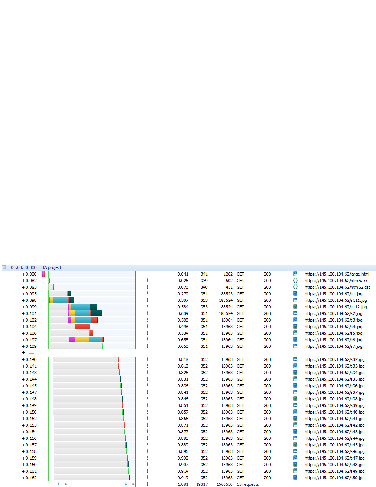
\includegraphics[scale=2]{images/http.pdf}
	\caption{Page Requests for large.html}
	\label{fig:httpwatch}
\end{figure}
  

It is essential to choose and implement the right tool to measure the response/request characteristics of the HTTP/1.1 and HTTP/2 protocol and to be able to compare them with each other. Thus, the bechmarking tool was chosen carefully and with respect to retrieve measurement data that can be used to compare both HTTP versions with each other. 
\\
H2load \cite{h2load} was the best candidate for that purpose. It has been developed to run test against HTTP/2 enabled webservers. i
It can also be used to conduct measurements against HTTP/1.1 enabled servers if, like in that case, a HTTP/2 - HTTP/1.1 reverse proxy is used taht is capable to translate HTTP/2 requests into HTTP/1.1 requests.    
